\documentclass[10pt]{article}
\usepackage[polish]{babel}
\usepackage[utf8]{inputenc}
\usepackage[T1]{fontenc}
\usepackage{amsmath}
\usepackage{amsfonts}
\usepackage{amssymb}
\usepackage[version=4]{mhchem}
\usepackage{stmaryrd}
\usepackage{graphicx}
\usepackage[export]{adjustbox}
\graphicspath{ {./images/} }

\title{Zadania - etap III \\
 (klasy 5 i 6 szkoły podstawowej) }

\author{}
\date{}


\begin{document}
\maketitle
Zadanie 1. Pewna liczba a przy dzieleniu przez 12 daje resztę 2, a inna liczba \(b\) przy dzieleniu przez 18 daje resztę 3. Jaką resztę przy dzieleniu przez 6 da liczba \(3 a+5 b\) ? Odpowiedź uzasadnij rachunkiem.

Zadanie 2. W kwadracie ABCD zawarty jest dwunastokąt o obwodzie 48 cm (rysunek poniżej). Każde dwa sąsiednie boki tego dwunastokąta są prostopadłe i równej długości. Oblicz pole kwadratu ABCD.\\
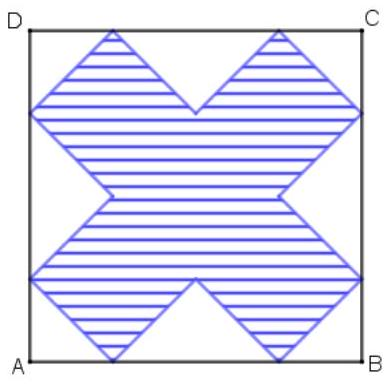
\includegraphics[max width=\textwidth, center]{2024_11_21_c870d62e3507162d8375g-1}

Zadanie 3. Szerokość pewnego prostokąta zwiększono o \(p \%\), gdzie \(p=\frac{2^{4}-2^{3}+0,25 \cdot 2^{3}}{(-1)-\left(-\frac{3}{2}\right)}\), a długość zmniejszono o \(30 \%\). Czy pole tego prostokąta zwiększyło się, czy zmniejszyło i o ile procent?

Zadanie 4. Znajdź ułamek o mianowniku 250, który jest większy od 0,49 lecz mniejszy od \(\frac{13}{25}\).\\
Zadanie 5. Na rysunku przedstawiono układ trójkątów równobocznych \(A, B, C, D, E, F\). Obwód trójkąta \(A\) jest równy 6 cm , zaś obwód trójkąta \(B\) jest równy 18 cm . Wyznacz sumę obwodów wszystkich narysowanych trójkątów.\\
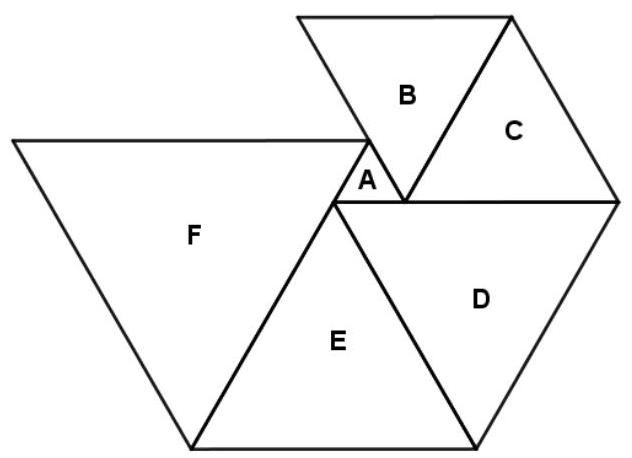
\includegraphics[max width=\textwidth, center]{2024_11_21_c870d62e3507162d8375g-1(1)}


\end{document}